\documentclass[10pt,a4paper]{article}

\usepackage[margin=1.8cm]{geometry}
\usepackage[T1]{fontenc}
\usepackage{mathptmx}
\usepackage{microtype}
\usepackage{graphicx}
\usepackage{booktabs}
\usepackage{amsmath}
\usepackage[font=small,labelfont=bf,skip=3pt]{caption}
\usepackage[numbers,sort&compress]{natbib}
\usepackage{enumitem}
\usepackage[compact]{titlesec}
\usepackage[colorlinks,urlcolor=blue,citecolor=black,linkcolor=black]{hyperref}

% --- compact layout for the 2-page limit ---
\titlespacing*{\section}{0pt}{6pt}{3pt}
\titlespacing*{\subsection}{0pt}{4pt}{2pt}
\setlist{nosep, leftmargin=*}
\setlength{\parskip}{2pt}
\setlength{\bibsep}{0pt}
\renewcommand{\bibfont}{\footnotesize}

\title{\vspace{-1.5cm}Biological Sequence Analysis -- Homework\\
       \large ORF prediction in bacteria and an HMM for eukaryotic gene finding}
\author{Idas Lukas Jasaitis}

\begin{document}
\maketitle



\section{Programming task: ORF prediction in bacterial genomes}
My script \texttt{orf\_finder.py} finds ORFs in a bacterial genome and then filters them
down to likely genes in four steps.

\begin{enumerate}
\item \textbf{Finding ORFs.} I search all six reading frames (three on each strand),
  because a gene can sit on either strand and start at any of three offsets. I use
  \href{https://www.ncbi.nlm.nih.gov/Taxonomy/Utils/wprintgc.cgi\#SG11}{NCBI genetic code 11},
  because it is the translation table for bacteria. I accept ATG, GTG and TTG as start
  codons, because some bacterial genes start with GTG or TTG and ATG alone would miss them.
  I keep one ORF per stop codon, starting at the most upstream start, because that is the
  usual definition of an ORF~\cite[\S3.5]{durbin1998}.

\item \textbf{Minimum length.} I set a separate cutoff for each genome instead of a fixed
  100 codons, because even random DNA has ORFs and how long they get depends on GC content.
  Stop codons are AT-rich, so random ORFs grow longer in GC-rich genomes~\cite{krogh_notes}.
  Following Problem~1.14 of the course problem book~\cite{borodovsky2006}, I treat each codon
  in random DNA as a stop with a fixed probability, which I compute from the genome's own
  base composition. I then keep only ORFs longer than 99\% of random ones.

\item \textbf{Codon-usage score.} I score ORFs by their codons, because genes prefer
  certain codons for the same amino acid while random ORFs do not~\cite[\S3.5]{durbin1998}.
  I learn codon frequencies from the longest half of the ORFs left after step~2, because
  ORFs that long are mostly real genes. Each ORF gets the sum of log-ratios between a
  codon's frequency in these genes and its frequency by chance, and I keep ORFs scoring
  above zero.

\item \textbf{Overlap filter.} I remove ORFs that overlap a better-scoring ORF by more than
  60\,bp, because a real gene also creates long ``shadow'' ORFs in other frames and on the
  other strand. Picking the best ORF first is a simpler, greedy version of what Prodigal
  does with dynamic programming~\cite{larralde2022}.
\end{enumerate}

\subsection{Results}
\begin{table}[h]
\centering\small
\caption{Results for three genomes of increasing GC content.}
\begin{tabular}{lrrrr}
\toprule
Genome & GC (\%) & Cutoff (codons) & ORFfinder ORFs & Predicted genes \\
\midrule
\textit{S.\ aureus} NCTC 8325 & 32.9 & 60  & 37\,264 & 2\,443 \\
\textit{E.\ coli} K-12 MG1655 & 50.8 & 99  & 78\,652 & 3\,661 \\
\textit{P.\ aeruginosa} PAO1  & 66.6 & 196 & 69\,936 & 3\,647 \\
\bottomrule
\end{tabular}
\end{table}
The cutoff rises with GC content as expected, and it is close to the classic 100 codons
only at 51\% GC. NCBI ORFfinder~\cite{orffinder} only lists ORFs (default minimum 75\,nt),
and it reports 15--21 times more ORFs than I predict as genes. \textit{P.\ aeruginosa} is
under-predicted, because at 67\% GC the cutoff drops every gene shorter than about 590\,nt.
The script also always takes the most upstream start, which is not always the real one.

TLDR: ORFfinder finds way more ORFs because it lists every ORF of 75\,nt or longer, accepts
more start codons and doesn't score or filter them further. I only added it to see a
comparison with another tool.

\section{HMM task: a model for eukaryotic gene finding}

\begin{figure}[h]
\centering
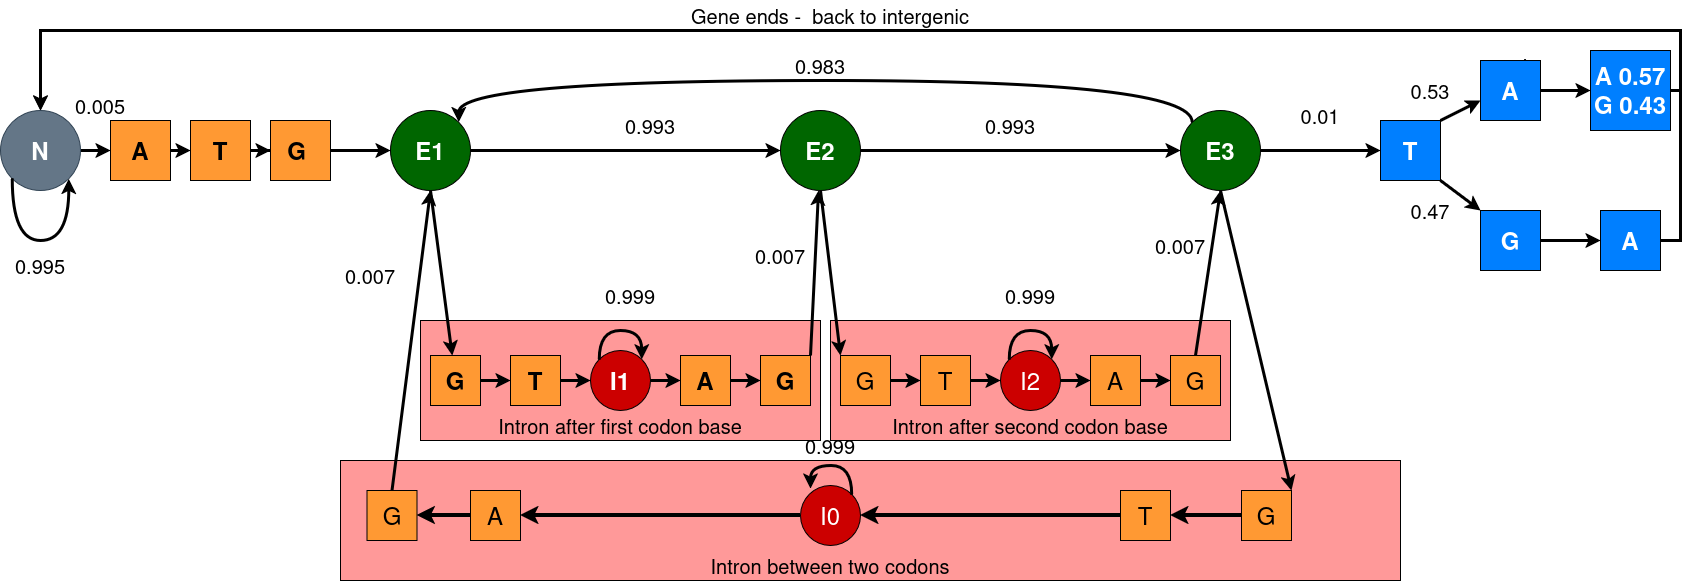
\includegraphics[width=\textwidth]{figures/hmm_gene_model.png}
\caption{HMM for eukaryotic gene finding (forward strand). Circles are states with their
own emission probabilities, boxes emit one fixed base. Numbers are illustrative transition
probabilities. Made with draw.io}
\label{fig:hmm}
\end{figure}

For this task I mainly relied on Durbin et al.~\cite{durbin1998}, chapter 3. In my model,
the hidden states are the parts of a gene (between genes, exon, intron) and what we observe
is the DNA sequence (Fig.~\ref{fig:hmm}). I only connected states in ways that happen in
real genes, because HMMs where every state connects to every other train badly.
\begin{enumerate}
\item \textbf{Between genes (N).} This state repeats itself for the DNA between genes. After
  each gene the model comes back here, so one sequence can contain many genes.
\item \textbf{Start codon.} Three states that always give A, T and G, because eukaryotic
  genes start with ATG.
\item \textbf{Exons.} One state for each position in a codon (E1, E2, E3), because the first,
  second and third bases of codons have different base frequencies. After E3 the model goes
  back to E1 for the next codon.
\item \textbf{Introns.} An intron can split a codon after its first, second or third base,
  so I made three intron copies. Each one goes back to the right codon position, so the
  codons still line up after the intron. Introns start with GT and end with AG, so these
  bases are fixed states.
\item \textbf{Stop codon.} The stop states are split into branches so they can only make
  TAA, TAG or TGA. Then the model goes back to N.
\end{enumerate}

\textbf{Probabilities.} The numbers in Fig.~\ref{fig:hmm} are example values, not measured
ones. A high self-loop probability, such as 0.999 for introns, means the model stays in that
state for a long stretch of DNA. Real values would be counted from genes that are already
annotated.

\section{Github}
\href{https://github.com/ChlorIdas/homework_1_BSA}{GitHub}    

\bibliographystyle{unsrtnat}
\bibliography{references}

\end{document}